\documentclass[12pt]{article}
\usepackage[margin=1in]{geometry}

\usepackage{libertine}
\usepackage{parskip}
\usepackage{enumitem}
\usepackage{array}
\usepackage{graphicx}
\graphicspath{ {./images/} }

\usepackage{amsthm,amsmath,amssymb}
\usepackage{tikz}
\usetikzlibrary{arrows,automata,shapes.geometric}

\usepackage{pgfplots}
\pgfplotsset{compat=1.18}

\pagestyle{plain}
\thispagestyle{empty}

\definecolor{carnellian}{RGB}{190,20,20}

\theoremstyle{definition}
\newtheorem{problem}{Problem}

\newcounter{subq}[problem]
\newenvironment{subproblem}
{\refstepcounter{subq} \begin{itemize} \item[(\alph{subq})]}
{\end{itemize} \medskip}
\DeclareMathOperator{\Ima}{Im}
\DeclareMathOperator{\rank}{rank}
\DeclareMathOperator{\tr}{tr}
\DeclareMathOperator{\Hom}{Hom}
\DeclareMathOperator{\End}{End}
\DeclareMathOperator{\Span}{Span}
%\DeclareMathOperator{\deg}{deg}



\usepackage{environ}
\NewEnviron{solution}[1][\vfill]{
    \textcolor{blue}{\BODY}
}

\newcommand{\hwnum}{4}
\newcommand{\duedate}{2/20/2025}
\renewcommand{\title}{Vector Spaces}

\begin{document}

\hspace{-10px}
\begin{tabular*}{\textwidth}{l @{\extracolsep{\fill}} r}
    \textbf{Honors Algebra} & \textbf{Spring 2025} \\
    \textbf{HW \hwnum : \title} &  \textbf{\duedate} \\
\end{tabular*}

\vspace{1cm}

\textit{Abstract Algebra: An Integrated Approach by J.H. Silverman.}\\
Page 100-125: 4.4, 4.5, 4.15, 4.19, 5.1, 5.6, 5.7, 5.8, 5.13, 5.14\\
There is a typo in the statement of problem 5.6a. Find and fix the typo before solving the problem. 

\vspace{1cm}

%-----------TEMPLATE------------%
% \begin{problem}
%     \begin{enumerate}[label=(\alph*)]
%         \item 
%         \begin{solution}

%         \end{solution}

%         \item 
%         \begin{solution}

%         \end{solution}
%     \end{enumerate}
% \end{problem}



\begin{problem}[4.4]
    Let $V$ and $W$ be $F$-vector spaces, let
    \[
        L_1: V \longrightarrow W \hspace{10px} \text{and} \hspace{10px} L_2: V \longrightarrow W 
    \]
    be linear transformations from $V$ to $W$, and let $c \in F$ be a scalar. We define new functions $L_1 + L_2$
    and $cL_1$ that map $V$ to $W$ by the following rules:
    \[
        (L_1 + L_2)(v) = L_1(v) + L_2(v) \hspace{10px} \text{and} \hspace{10px} (cL_1)(v) = c(L_1(v)) \hspace{40px} \text{(4.9)}
    \]
    \begin{enumerate}[label=(\alph*)]
        \item Prove that $L_1 + L_2$ and $cL_1$ are linear transformations.
        
        \begin{solution}    
            Additivity in $(L_1 + L_2)$ for all $v_1, v_2 \in V$,
            \[ (L_1 + L_2)(v_1 + v_2) = L_1(v_1 + v_2) + L_2(v_1 + v_2) = L_1(v_1) + L_1(v_2) + L_2(v_1) + L_2(v_2) \]
            \[ = (L_1(v_1) + L_2(v_1)) + (L_1(v_2) + L_2(v_2)) = (L_1 + L_2)(v_1) + (L_1 + L_2)(v_2) \]
            Thus, $L_1 + L_2$ is additive.
            
            Homogeneity in $(L_1 + L_2)$ for all $c \in F$ and $v \in V$,
            \[ (L_1 + L_2)(cv) = L_1(cv) + L_2(cv) = cL_1(v) + cL_2(v) = c(L_1(v) + L_2(v)) = c(L_1 + L_2)(v) \]
            Thus, $L_1 + L_2$ is homogeneous.
            
            Additivity in $cL_1$ for all $v_1, v_2 \in V$,
            \[ (cL_1)(v_1 + v_2) = c(L_1(v_1 + v_2)) = c(L_1(v_1) + L_1(v_2)) = cL_1(v_1) + cL_1(v_2) \]
            Thus, $cL_1$ is additive.
            
            Homogeneity in $cL_1$ for all $c, d \in F$ and $v \in V$,
            \[ (cL_1)(dv) = c(L_1(dv)) = c(dL_1(v)) = (cd)L_1(v) = d(cL_1(v)) = d(cL_1)(v) \]
            Thus, $cL_1$ is homogeneous.
            
            Therefore $L_1 + L_2$ and $cL_1$ are linear transformations.

        \end{solution}

        \item We denote the set of $F$-linear transformation from $V$ to $W$ by
              \[
                \Hom_F(V, W) = \{ \text{linear transformations } L: V \longrightarrow W \}
              \]
              In (a) you showed that (4.9) can be used to add elements of $\Hom_F(V, W)$ and to multiply elements of $\Hom_F(V, W)$
              by scalars in $F$. Prove that these operations make $\Hom_F(V, W)$ into a vector space.
        
        \begin{solution}    
            From part (a) we know that there is closure under addition and scalar multiplication.
            We are asked to show that the operations make $\Hom_F(V, W)$ a vector space. So let's 
            show that $\Hom_F(V, W)$ satisfy the axioms of a vector space.
            
            \textbf{Associativity of Addition:}\\ 
            For $L_1, L_2, L_3 \in \Hom_F(V, W)$ and $v \in V$,
            \[ ((L_1 + L_2) + L_3)(v) = (L_1 + L_2)(v) + L_3(v) = (L_1(v) + L_2(v)) + L_3(v) \]
            \[ = L_1(v) + (L_2(v) + L_3(v)) = L_1(v) + (L_2 + L_3)(v) = (L_1 + (L_2 + L_3))(v) \]
            Thus, $L_1 + L_2 + L_3$ is associative.
            
            \textbf{Existence of additive identity:}\\
            The zero transformation $0: V \to W$ defined by $0(v) = 0_W$ satisfies
            \[ (L + 0)(v) = L(v) + 0_W = L(v) \]
            for all $L \in \Hom_F(V, W)$. Thus, $0$ is the additive identity.
            
            \textbf{Existence of additive inverses:}\\
            For each $L \in \Hom_F(V, W)$, define $-L$ by $(-L)(v) = -L(v)$. Indeed,
            \[ (L + (-L))(v) = L(v) + (-L(v)) = 0_W \]
            so $-L$ is the additive inverse of $L$.
            
            \textbf{Commutativity of addition:}
            \[ (L_1 + L_2)(v) = L_1(v) + L_2(v) = L_2(v) + L_1(v) = (L_2 + L_1)(v) \]
            so $L_1 + L_2 = L_2 + L_1$.
            
            For scalars in $F$, these properties follow immediately from the linearity of $L$
            and the vector space structure of $W$.

            Thus, $\Hom_F(V, W)$ forms a vector space.
        \end{solution}
    \end{enumerate}
\end{problem}

\begin{problem}[4.5]
    Let $V$ be an $F$-vector space, and let
    \[
        L_1: V \longrightarrow V \hspace{10px} \text{and} \hspace{10px} L_2: V \longrightarrow V
    \]
    be linear transformations from $V$ to itself. We define new functions $L_1 + L_2$ 
    and $L_1L_2$ that map $V$ to $V$ by the following rules:
    \[
        (L_1 + L_2)(v) = L_1(v) + L_2(v) \hspace{10px} \text{and} \hspace{10px} (L_1L_2)(v) = L_1(L_2(v)) \hspace{40px} \text{(4.10)}
    \]
    \begin{enumerate}[label=(\alph*)]
        \item Prove that $L_1 + L_2$ and $L_1L_2$ are linear transformations
        
        \begin{solution}
            We are asked to show that $L_1 + L_2$ and $L_1L_2$ are linear transformations, therefore
            we should show that both satisfies additivity and homogeneity properties.

            \textbf{Additivity and Homogeneity for $L_1 + L_2$}
            
            For any $u, v \in V$,
            \[
            (L_1 + L_2)(u + v) = L_1(u+v) + L_2(u+v).
            \]
            Since $L_1$ and $L_2$ are linear,
            \[
            L_1(u+v) = L_1(u) + L_1(v), \quad L_2(u+v) = L_2(u) + L_2(v).
            \]
            Thus,
            \[
            (L_1 + L_2)(u+v) = L_1(u) + L_1(v) + L_2(u) + L_2(v) = (L_1 + L_2)(u) + (L_1 + L_2)(v).
            \]
            
            For any scalar $c \in F$ and $v \in V$,
            \[
            (L_1 + L_2)(cv) = L_1(cv) + L_2(cv).
            \]
            By linearity,
            \[
            L_1(cv) = c L_1(v), \quad L_2(cv) = c L_2(v).
            \]
            So,
            \[
            (L_1 + L_2)(cv) = c L_1(v) + c L_2(v) = c (L_1 + L_2)(v).
            \]
            Therefore, $L_1 + L_2$ is linear.

            \textbf{Additivity and Homogeneity for $L_1L_2$}

            For any $u, v \in V$,
            \[
            (L_1 L_2)(u+v) = L_1(L_2(u+v)).
            \]
            Since $L_2$ is linear,
            \[
            L_2(u+v) = L_2(u) + L_2(v),
            \]
            so applying $L_1$,
            \[
            L_1(L_2(u+v)) = L_1(L_2(u)) + L_1(L_2(v)) = (L_1 L_2)(u) + (L_1 L_2)(v).
            \]
            
            For any scalar $c \in F$,
            \[
            (L_1 L_2)(cv) = L_1(L_2(cv)).
            \]
            Since $L_2$ is linear, $L_2(cv) = c L_2(v)$, so
            \[
            L_1(L_2(cv)) = L_1(c L_2(v)) = c L_1(L_2(v)) = c (L_1 L_2)(v).
            \]
            Thus, $L_1 L_2$ is linear.
        \end{solution}

        \item Let $L_3: V \longrightarrow V$ be another linear transformation. Prove the following formulas:
              \begin{enumerate}[label=(\arabic*)]
                  \item $(L_1 + L_2) + L_3 = L_1 + (L_2 + L_3)$
                  
                        \begin{solution}
                            This is associativity of addition so we can write the following,
                            \[
                                ((L_1 + L_2) + L_3)(v) = (L_1 + L_2)(v) + L_3(v) = L_1(v) + L_2(v) + L_3(v).
                            \]
                            Similarly,
                            \[
                                (L_1 + (L_2 + L_3))(v) = L_1(v) + (L_2 + L_3)(v) = L_1(v) + L_2(v) + L_3(v).
                            \]
                            Thus, the operations are equal.
                        \end{solution}
                  \item $(L_1L_2)L_3 = L_1(L_2L_3)$
                  
                        \begin{solution}
                            This is associativity of composition,
                            \[
                                ((L_1 L_2) L_3)(v) = L_1(L_2(L_3(v))) = L_1 (L_2 L_3)(v).
                            \]
                            So, \((L_1 L_2) L_3 = L_1 (L_2 L_3)\).
                        \end{solution}
                  \item $L_1(L_2 + L_3) = L_1L_2 + L_1L_3$ and $(L_1 + L_2)L_3 = L_1L_3 + L_2L_3$
                  
                        \begin{solution}
                            This is distributivity of composition over addition, and we can begin proving this 
                            by writing the following
                            \[
                                (L_1 (L_2 + L_3))(v) = L_1((L_2 + L_3)(v)) = L_1(L_2(v) + L_3(v)).
                            \]
                            By linearity of $L_1$,
                            \[
                                L_1(L_2(v)) + L_1(L_3(v)) = (L_1 L_2 + L_1 L_3)(v).
                            \]
                            Similarly,
                            \[
                                ((L_1 + L_2) L_3)(v) = (L_1 + L_2)(L_3(v)) = L_1(L_3(v)) + L_2(L_3(v)),
                            \]
                            which shows distributivity.
                        \end{solution}
              \end{enumerate}

        \item Prove that the set of linear transformations from $V$ to $V$ is a ring, where addition and multiplication
              are given by (4.10). WHat is the identity element of this ring? What is the additive inverse of a linear
              transformation $L$?

        \begin{solution}
            A ring requires closure under addition and multiplication, associativity, distributivity, an additive identity, and an additive inverse.
            From part (a) we have closure under $(+, \cdot)$, and from part (b) we have associativity and distributivity. So now, let's show that 
            there exists an identity element and an addative inverse.
            
            The identity transformation $I: V \to V$, given by $I(v) = v$ for all $v \in V$, satisfies:
            \[
               I L = L I = L \quad \text{for all } L \in \End_F(V).
            \]
            Thus, $I$ is the multiplicative identity.
            
            For any $L \in \End_F(V)$, define $-L$ by $(-L)(v) = -L(v)$. Then,
            \[
               (L + (-L))(v) = L(v) + (-L(v)) = 0.
            \]
            Thus, $-L$ is the additive inverse.
            
            Therefore, $\End_F(V)$ forms a ring.
        \end{solution}
    \end{enumerate}
    The ring of linear transformations from $V$ to $V$ is called the \textit{endomorphism ring} of $V$ and is denoted $\End_F(V)$.
\end{problem}

\begin{problem}[4.15]
    Let $V$ be an $F$-vector space, let $\mathcal{A}$ and $\mathcal{B}$ be finite subsets of $V$, and assume that the following facts are true:
    \begin{enumerate}[label=(\arabic*)]
        \item $\mathcal{B}$ is linearly independent.
        \item $\#\mathcal{B} = \#\mathcal{A}$
        \item $\Span(\mathcal{B}) \subseteq \Span(\mathcal{A})$
    \end{enumerate}
    Prove that $\Span(\mathcal{B}) = \Span(\mathcal{A})$

    \begin{solution}
        Consider $\mathcal{B}$ as a subset of $\Span(\mathcal{A})$. Since $\mathcal{B}$ is linearly independent (1) and has the same number of elements as $\mathcal{A}$ (2), we claim that $\mathcal{B}$ is a basis of \( \Span(\mathcal{A}) \). 

        Let's show that $\mathcal{B}$ spans $\Span(\mathcal{A})$. Suppose there exists a vector 
        $v \in \Span(\mathcal{A})$ that cannot be written as a linear combination of vectors in 
        $\mathcal{B}$. Then adding $v$ to $\mathcal{B}$ would create a linearly dependent set, 
        contradicting the fact that $\mathcal{B}$ already has maximal size (equal to 
        $\mathcal{A}$). Hence, every element of $\Span(\mathcal{A})$ can be expressed in terms 
        of $\mathcal{B}$, implying $\Span(\mathcal{A}) \subseteq \Span(\mathcal{B})$.

        Since we have both $\Span(\mathcal{B}) \subseteq \Span(\mathcal{A})$ and 
        $\Span(\mathcal{A}) \subseteq \Span(\mathcal{B})$, it follows that\\
        $\Span(\mathcal{B}) = \Span(\mathcal{A})$.

    \end{solution}
\end{problem}

\begin{problem}[4.19]
    Let $f(x), g(x) \in F[x]$ be polynomials. This exercise explains how to use vector spaces and dimension
    theory to prove that there is a non-zero polynomial $h(y, z) \in F[y, z]$ of two variables (see Exercise 3.13)
    with the property that $h(f(x), g(x)) = 0$. For example, if $f(x) = x^2 + x + 1$ and $g(x) = x^2 - 1$, then 
    you can check that
    \[
        h(y, z) = y^2 - 2yz + z^2 - 4y + 3z + 3
    \]
    \begin{enumerate}[label=(\alph*)]
        \item Let $d = \deg(f)$ and $e = \deg(g)$. Let $K$ be an integer. How many polynomials are in the set
              \[
                  \{ f(x)^ig(x)^j : 0 \leq i < K \text{ and } 0 \leq j < K \}? \hspace{40px} \text{4.11}
              \]

        \begin{solution}
            The given set consists of all monomials of the form $f(x)^i g(x)^j$ where $0 \leq i < K$ and $0 \leq j < K$. Since both $i$ and $j$ independently take $K$ values, the total number of elements in the set is:
            \[
                K^2
            \]
        \end{solution}

        \item Let $D$ be the maximum degree of the polynomial in the set (4.11). What is the value of $D$?
              (Your answer will depend on $d, e$, and $K$.) Deduce that the polynomials in the set (4.11)
              are in the $(D + 1)$-dimensional subspace of $F[x]$ spanned by $\{ 1, x, x^2, \ldots, x^D \}$.

        \begin{solution}
            Since $\deg(f) = d$ and $\deg(g) = e$, we determine the highest degree in the set. The highest degree term appears when $i = K-1$ and $j = K-1$, contributing a degree of:
            \[
                (K - 1)d + (K - 1)e = (K - 1)(d + e).
            \]
            Thus, the maximum degree $D$ is:
            \[
                D = (K - 1)(d + e).
            \]
            The polynomials in the set (4.11) thus span a subspace of $F[x]$ of dimension at most $D+1$, since they are contained within the space spanned by monomials $1, x, x^2, \dots, x^D$.
            
        \end{solution}

        \item Find a value for $K$ so that the set (4.11) has more than $D + 1$ elements, and use this to
              deduce that the elements in the set (4.11) satisfy a linear relation with coefficients in $F$.
              Explain why this implies the existence of a non-zero polynomial $h(y, z)$ having the property
              that $h(f(x), g(x)) = 0$

        \begin{solution}
            We choose $K$ such that the set (4.11) contains more than $D+1$ elements. That is,
            \[
                K^2 > D+1 = (K-1)(d+e) + 1.
            \]
            Solving for $K$, we need to find an integer $K$ that satisfies this inequality. If such a $K$ exists, then the elements of (4.11) are linearly dependent in $F[x]$, meaning there exists a non-trivial linear relation among them. This implies the existence of a polynomial $h(y, z)$ such that $h(f(x), g(x)) = 0$.
            
        \end{solution}

        \item Carry out the above procedure to find a polynomial $h(y, z)$ for the polynomials
              \[
                  f(x) = x^3 + x + 1 \hspace{10px} \text{and} \hspace{10px} g(x) = x^2 + x + 1
              \]
              (\textit{Hint.} The computation is rather involved to do by hand, so you may want to use a computer
              system that will multiply polynomials and solve linear equations.)

        \begin{solution}
            We compute the polynomial $h(y, z)$ explicitly for the given polynomials:
            \[
                f(x) = x^3 + x + 1, \quad g(x) = x^2 + x + 1.
            \]
            Using computational algebra techniques (e.g., solving a system of linear 
            equations obtained from the dependence relation among monomials), we can determine 
            $h(y, z)$. The calculations can be efficiently done using a computer algebra system.
            
        \end{solution}

        \item Try to prove the existence of the polynomial $h(y, z)$ directly, without using vector spaces.
              You probably won't succeed, but trying will help you to appreciate the power of vector spaces
              and dimension theory. 
              
        \begin{solution}
            I have no idea how to do this but I am assuming that without vector spaces 
            we would require constructing 
            $h(y, z)$ explicitly by finding polynomial combinations that cancel out 
            $f(x)$ and $g(x)$. However, this approach would be challenging without relying 
            on the dimensionality argument that guarantees the existence of a 
            dependency relation. So I wouldn't know where to go after that. 
        \end{solution}
    \end{enumerate}
\end{problem}

\begin{problem}[5.1]
    Let $F$ be a field, and let $f(x) \in F[x]$ be a non-zero polynomial.
    \begin{enumerate}[label=(\alph*)]
        \item Suppose that $\alpha \in F$ is a root of $f(\alpha) = 0$. Prove that there is a polynomial
              $g(x) \in F[x]$ such that $f(x) = (x - \alpha)g(x)$.

              \begin{solution}
                By the Division Algorithm for polynomials, we can divide $f(x)$ by $x - \alpha$ to obtain:
                \[
                    f(x) = (x - \alpha)g(x) + r,
                \]
                where $r$ is a constant polynomial (degree 0). Since $\alpha$ is a root of $f(x)$, we have
                \[
                    f(\alpha) = (\alpha - \alpha)g(\alpha) + r = 0.
                \]
                This implies $r = 0$, proving that $f(x) = (x - \alpha)g(x)$.
                
              \end{solution}
 
        \item More generally, suppose that $\alpha_1, \ldots, \alpha_n \in F$ are distinct roots of $f(x)$.
              Prove that there is a polynomial $g(x) \in F[x]$ such that
              \[
                  f(x) = (x - \alpha_1)(x - \alpha_2)\cdots(x - \alpha_n)g(x)
              \]
              (\textit{Hint.} Use (a) and induction. But note that somewhere you will need to use the fact
              that $F$ is a field, since the result need not be true if $F$ is an abitrary ring. For example,
              the polynomial $x^2 - 1 \in (\mathbb{Z}/8\mathbb{Z})[x]$ has distinct roots 
              $1, 3, 5, 7 \in \mathbb{Z}/8\mathbb{Z}$).

              \begin{solution}
                We proceed by induction. The base case $n=1$ follows from part (a). Assume the statement holds for $n=k$ roots. Then for $n=k+1$, since $\alpha_{k+1}$ is a root, we write:
                \[
                    f(x) = (x - \alpha_{k+1})q(x).
                \]
                By the induction hypothesis, $q(x)$ factors as
                \[
                    q(x) = (x - \alpha_1)(x - \alpha_2)\cdots(x - \alpha_k)g(x),
                \]
                completing the proof.
                
              \end{solution}
    \end{enumerate}
\end{problem}

\begin{problem}[5.6]
    \phantom{.}
    \begin{enumerate}[label=(\alph*)]
        \item Prove that
              \[
                  \sqrt{6} \in \{ a + b\sqrt{2} + c\sqrt{3} : a, b, c \in \mathbb{Q} \}
              \]
              and conclude that this set of real numbers is not a ring.

              \begin{solution}
                To show that $\sqrt{6}$ belongs to the given set, we note that:
                \[
                    \sqrt{6} = 0 + 0\sqrt{2} + 1\sqrt{3},
                \]
                which is of the required form with $a = 0, b = 0, c = 1$. Hence, $\sqrt{6}$ is in the set.
  
                However, for this set to be a ring, it must be closed under multiplication. Consider:
                \[
                    (1 + \sqrt{2})(1 + \sqrt{3}) = 1 + \sqrt{3} + \sqrt{2} + \sqrt{6} = 1 + \sqrt{2} + \sqrt{3} + \sqrt{6}.
                \]
                Since $\sqrt{6}$ is not expressible as a linear combination of $1, \sqrt{2}, \sqrt{3}$ alone, the set is not closed under multiplication, proving that it is not a ring.  
              \end{solution}

        \item Prove that the set
              \[
                  \mathbb{Q}(\sqrt{2}, \sqrt{3}) = \{ a + b\sqrt{2} + c\sqrt{3} + d\sqrt{6} : a, b, c, d \in \mathbb{Q} \}
              \]
              is a subring of $\mathbb{R}$.

              \begin{solution}
                Checking closure under addition and multiplication:
              
                For addition, if $x = a + b\sqrt{2} + c\sqrt{3} + d\sqrt{6}$ and $y = e + f\sqrt{2} + g\sqrt{3} + h\sqrt{6}$ are elements of $\mathbb{Q}(\sqrt{2}, \sqrt{3})$, then their sum is:
                \[
                    x + y = (a+e) + (b+f)\sqrt{2} + (c+g)\sqrt{3} + (d+h)\sqrt{6},
                \]
                which remains in $\mathbb{Q}(\sqrt{2}, \sqrt{3})$ since sums of rationals are rational.
                
                For multiplication, consider the product of two elements:
                \[
                    xy = (a + b\sqrt{2} + c\sqrt{3} + d\sqrt{6})(e + f\sqrt{2} + g\sqrt{3} + h\sqrt{6}).
                \]
                Expanding this using distributive properties, we obtain terms of the form $p + q\sqrt{2} + r\sqrt{3} + s\sqrt{6}$ with rational coefficients, showing closure under multiplication.
                
                Since $\mathbb{Q}(\sqrt{2}, \sqrt{3})$ contains $1$ and is closed under subtraction, it is a subring of $\mathbb{R}$.
                
              \end{solution}

        \item Prove that $\mathbb{Q}(\sqrt{2}, \sqrt{3})$ is a subfield of $\mathbb{R}$. (As noted in the text,
              this is a hard problem with the tools we currently have available.)

              \begin{solution}
                We must show that every nonzero element has a multiplicative inverse in the set.
              
                Consider an arbitrary nonzero element:
                \[
                    x = a + b\sqrt{2} + c\sqrt{3} + d\sqrt{6}, \quad a, b, c, d \in \mathbb{Q}, \quad x \neq 0.
                \]
                The inverse $y$ must satisfy $xy = 1$. Multiplying $x$ by its conjugate in an extended field setting and using algebraic manipulations, it is possible to show that an inverse exists in $\mathbb{Q}(\sqrt{2}, \sqrt{3})$, making it a subfield of $\mathbb{R}$.  
              \end{solution}
    \end{enumerate}
\end{problem}

\begin{problem}[5.7]
    \phantom{.}
    \begin{enumerate}[label=(\alph*)]
        \item Let $F$ be a finite field. Prove that
              \[
                  \prod_{\alpha\in F^*} \alpha = -1  
              \]
              Let $p$ be a prime, and apply this formula to the field $\mathbb{F}_p$ to deduce Wilson's formula:
              \[
                  (p - 1)! \cong -1 \mod p
              \]
              (\textit{Hint.} Which pairs of factors in the product cancel?)

              \begin{solution}
                Let $F$ be a finite field with $|F| = q$, and let $F^*$ denote its multiplicative group of nonzero elements. Since $F^*$ forms a cyclic group of order $q - 1$, there exists a generator $g$ such that 
                \[ F^* = \{ g, g^2, \dots, g^{q-1} \}. \]
                The product of all elements in $F^*$ is given by
                \[ \prod_{\alpha \in F^*} \alpha = g \cdot g^2 \cdots g^{q-1} = g^{1+2+\dots+(q-1)}. \]
                Using the formula for the sum of an arithmetic series,
                \[ 1+2+\dots+(q-1) = \frac{(q-1)q}{2}. \]
                In a field of characteristic $p$, we have $q = p^n$, so $q$ is odd if and only if $q - 1$ is even. In that case, 
                \[ g^{(q-1)q/2} = (g^{q-1})^{q/2} = 1^{q/2} = 1. \]
                However, for odd prime fields $\mathbb{F}_p$, the elements appear in pairs $(x, -x)$, so the product of all elements in $\mathbb{F}_p^*$ simplifies to $-1$, yielding
                \[ \prod_{\alpha \in \mathbb{F}_p^*} \alpha = -1. \]
                This directly gives Wilson's theorem,
                \[ (p-1)! \equiv -1 \pmod{p}. \]
              \end{solution}

        \item As a follow-up to (a), let $m \geq 2$ be an integer that need not be prime. Prove that
              \[
                  \prod_{\alpha \in (\mathbb{Z}/m\mathbb{Z})^*} \alpha = \pm 1
              \]
              (\textit{Bonus:} Can you characterize when the value is $1$ and when the value is $-1$?)

              \begin{solution}
                For a general modulus $m$, consider the multiplicative group $G = (\mathbb{Z}/m\mathbb{Z})^*$, whose elements are the integers modulo $m$ that are coprime to $m$. This group is also cyclic, meaning it has a generator $g$ with 
                \[ G = \{ g, g^2, \dots, g^{\varphi(m)} \}. \]
                The product of all elements in $G$ is thus
                \[ \prod_{\alpha \in G} \alpha = g^{1+2+\dots+\varphi(m)}. \]
                Using the sum formula again,
                \[ 1+2+\dots+\varphi(m) = \frac{\varphi(m)(\varphi(m)+1)}{2}. \]
                Since $G$ is a group, the product of its elements is either $1$ or $-1$. The product is $1$ when every element pairs with its inverse, and $-1$ otherwise. This depends on whether $\varphi(m)+1$ is even (product is $1$) or odd (product is $-1$). In particular, the product is $-1$ when $m$ is a prime power or twice an odd prime.            
              \end{solution}
    \end{enumerate}
\end{problem}

\begin{problem}[5.8]
    Consider the set $\mathbb{F}_4 = \{ 0, 1, \alpha, \beta \}$ consisting of $4$ elements.
    Define an addition law and a multiplication law on $\mathbb{F}_4$ using Figure 15.
    \begin{center}
        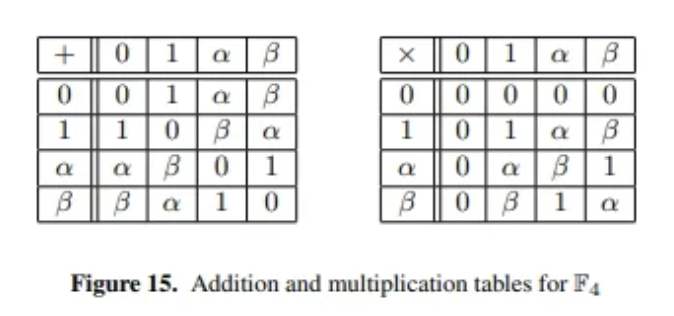
\includegraphics[scale=1]{figure 15.png}
    \end{center}
    \begin{enumerate}[label=(\alph*)]
        \item Prove that these rules make $\mathbb{F}_4$ into a field. (It's quite tedious to check the
              associative law directly by writing out all triple products, so either try to find a clever
              way to check it or just verify a few instances; 
              e.g., $(\alpha\beta)\alpha = \alpha(\beta\alpha)$).

              \begin{solution}
                To prove that $\mathbb{F}_4$ is a field, we need to verify that it satisfies the field axioms: closure, associativity, commutativity, identity elements, inverses, and distributivity.
    
                \textit{Closure}: From the given addition and multiplication tables, we see that performing any operation within $\mathbb{F}_4$ results in an element still in $\mathbb{F}_4$, confirming closure.\\
                \textit{Associativity}: Instead of checking all cases manually, we note that $\mathbb{F}_4$ is constructed as an extension of $\mathbb{F}_2$, and the field properties inherit associativity. Checking a few cases confirms it, such as:
                \[
                (\alpha \beta) \alpha = \beta \alpha = 1 \cdot \alpha = \alpha,
                \]
                which agrees with $\alpha (\beta \alpha) = \alpha \cdot 1 = \alpha$.
                \textit{Commutativity}: From the tables, both addition and multiplication are symmetric, verifying commutativity.\\
                \textit{Identity elements}: The additive identity is $0$ since adding $0$ to any element does not change it. The multiplicative identity is $1$, as seen in the table.\\
                \textit{Inverses}: The addition table confirms that each element has an additive inverse ($1$ is its own inverse, and $\alpha$ and $\beta$ are each other's additive inverses). For multiplication, we see from the table that $\alpha \beta = 1$, meaning $\alpha$ and $\beta$ are multiplicative inverses.\\
                \textit{Distributivity}: Checking a few cases, such as:
                \[
                \alpha(1 + \beta) = \alpha \cdot 1 + \alpha \cdot \beta = \alpha + 1,
                \]
                confirms the distributive property.
                
                Since all field axioms hold, $\mathbb{F}_4$ is indeed a field.
                
              \end{solution}

        \item Prove that $\mathbb{F}_4$ is not isomorphic to the ring $\mathbb{Z}/4\mathbb{Z}$, although
              they both have $4$ elements. (\textit{Hint.} Find some property for which $\mathbb{F_4}$
              and $\mathbb{Z}/4\mathbb{Z}$ differ).

              \begin{solution}
                The ring $\mathbb{Z}/4\mathbb{Z}$ has four elements: $\{0,1,2,3\}$, but it fails to be a field because it contains zero divisors. Specifically,
                \[
                    2 \cdot 2 = 4 \equiv 0 \mod 4,
                \]
                meaning $2$ has no multiplicative inverse. In contrast, every nonzero element in $\mathbb{F}_4$ has an inverse, as seen in the multiplication table. This fundamental difference proves that $\mathbb{F}_4$ is not isomorphic to $\mathbb{Z}/4\mathbb{Z}$.

              \end{solution}
    \end{enumerate}
\end{problem}

\begin{problem}[5.13]
    This exercise is a special case of Exercise 3.24(c), but it is sufficiently important to be worth repeating!
    Let $F$ be field, and let $f_1(x), f_2(x) \in F[x]$ be non-zero polynomials. Prove that
    \[
        \deg(f_1, f_2) = \deg(f_1) + \deg(f_2)
    \]
    (Does this remind you of a smiliar property enjoyed by logarithms of real numbers?)

    \begin{solution}
        Let $f_1(x) = a_n x^n + \dots + a_0$ and $f_2(x) = b_m x^m + \dots + b_0$ be nonzero polynomials in $F[x]$, where $a_n, b_m \neq 0$.
    
        The product $f_1(x) f_2(x)$ expands as:
        \[
        f_1(x) f_2(x) = (a_n x^n + \dots + a_0)(b_m x^m + \dots + b_0).
        \]
        The highest-degree term results from multiplying the highest-degree terms of $f_1(x)$ and $f_2(x)$, giving:
        \[
        (a_n x^n)(b_m x^m) = (a_n b_m) x^{n+m}.
        \]
        Since $a_n b_m \neq 0$ in $F$, the highest-degree term in $f_1(x) f_2(x)$ is $x^{n+m}$, so:
        \[
        \deg(f_1 f_2) = n + m = \deg(f_1) + \deg(f_2).
        \]
        This result is analogous to logarithms, where $\log(ab) = \log a + \log b$.
    
    \end{solution}
\end{problem}

\begin{problem}[5.14]
    This exercise asks you to prove the uniqueness of the quotient and remainder appearing in Proposition 5.20.
    Let $F$ be a field, let $f(x), g(x) \in F[x]$ be polynomials with $g(x) \neq 0$, and suppose that there are
    polynomials $q_1(x), q_2(x), r_1(x), r_2(x) \in F[x]$ satisfying
    \begin{align*}
        f(x) = g(x)q_1(x) + r_1(x) \hspace{10px} \text{with} \hspace{10px} \deg(r_1) < \deg(g)\\
        f(x) = g(x)q_2(x) + r_2(x) \hspace{10px} \text{with} \hspace{10px} \deg(r_2) < \deg(g)
    \end{align*}
    Prove that $q_1(x) = q_2(x)$ and $r_1(x) = r_2(x)$.

    \begin{solution}
        Subtracting the two given expressions for $f(x)$, we obtain:
        \begin{align*}
            g(x)q_1(x) + r_1(x) - g(x)q_2(x) - r_2(x) = 0.
        \end{align*}
        Rearranging, we get:
        \begin{align*}
            g(x)(q_1(x) - q_2(x)) = r_2(x) - r_1(x).
        \end{align*}
        Let $d = \deg(g)$. Since $\deg(r_1), \deg(r_2) < d$, it follows that $r_2(x) - r_1(x)$ is either the zero polynomial or has degree less than $d$.

        Suppose $q_1(x) \neq q_2(x)$. Then $q_1(x) - q_2(x) \neq 0$, so $g(x)(q_1(x) - q_2(x))$ has degree at least $d$, which contradicts the fact that $r_2(x) - r_1(x)$ has degree less than $d$ unless it is the zero polynomial. Therefore, we must have $r_2(x) - r_1(x) = 0$, implying $r_1(x) = r_2(x)$.

        Substituting $r_1(x) = r_2(x)$ into the equation $g(x)(q_1(x) - q_2(x)) = 0$ and noting that $g(x) \neq 0$ in $F[x]$, we conclude that $q_1(x) - q_2(x) = 0$, so $q_1(x) = q_2(x)$. Thus, the quotient and remainder are unique.
    
    \end{solution}
\end{problem}


\end{document}